\documentclass{article}
\usepackage{listings}
\usepackage{caption}
\usepackage{subcaption}
\usepackage{listings}
\usepackage{color}
\usepackage{hyperref}
\usepackage{graphicx}
\graphicspath{ {./} }
\usepackage[top=1in, bottom=1.25in, left=1.25in, right=1.25in]{geometry}
\definecolor{mygreen}{rgb}{0,0.6,0}
\definecolor{mygray}{rgb}{0.5,0.5,0.5}
\definecolor{mymauve}{rgb}{0.58,0,0.82}
\lstset{ %
	backgroundcolor=\color{white},   % choose the background color; you must add \usepackage{color} or \usepackage{xcolor}; should come as last argument
	basicstyle=\footnotesize,        % the size of the fonts that are used for the code
	breakatwhitespace=false,         % sets if automatic breaks should only happen at whitespace
	breaklines=true,                 % sets automatic line breaking
	captionpos=b,                    % sets the caption-position to bottom
	commentstyle=\color{mygreen},    % comment style
	deletekeywords={...},            % if you want to delete keywords from the given language
	escapeinside={\%*}{*)},          % if you want to add LaTeX within your code
	extendedchars=true,              % lets you use non-ASCII characters; for 8-bits encodings only, does not work with UTF-8
	frame=single,	                   % adds a frame around the code
	keepspaces=true,                 % keeps spaces in text, useful for keeping indentation of code (possibly needs columns=flexible)
	keywordstyle=\color{blue},       % keyword style
	language=Octave,                 % the language of the code
	morekeywords={*,...},            % if you want to add more keywords to the set
	numbers=left,                    % where to put the line-numbers; possible values are (none, left, right)
	numbersep=5pt,                   % how far the line-numbers are from the code
	numberstyle=\tiny\color{mygray}, % the style that is used for the line-numbers
	rulecolor=\color{black},         % if not set, the frame-color may be changed on line-breaks within not-black text (e.g. comments (green here))
	showspaces=false,                % show spaces everywhere adding particular underscores; it overrides 'showstringspaces'
	showstringspaces=false,          % underline spaces within strings only
	showtabs=false,                  % show tabs within strings adding particular underscores
	stepnumber=2,                    % the step between two line-numbers. If it's 1, each line will be numbered
	stringstyle=\color{mymauve},     % string literal style
	tabsize=2,	                   % sets default tabsize to 2 spaces
	title=\lstname                   % show the filename of files included with \lstinputlisting; also try caption instead of title
}
\author{Polykarpos Thomadakis}
\title{Assignment 4 \\
	\large CS834 Introduction to Information Retrieval\\Fall 2017}
	
\begin{document}
\maketitle
\section*{Question 10.3}
Compute five iterations of HITS (see Algorithm 3) and PageRank (see Figure 4.11) on the graph in Figure 10.3. Discuss how the PageRank scores compare to the hub and authority scores produced by HITS.
\subsection*{Answer}
For the purposes of this assignment I wrote a script that computes the values desired based on the algorithms provided in the book. First I create 2 classes that represent a node in the graph and the graph itself. Then I use them to run the HITS and PageRank algorithms on the graph. The output is a set of files that are then used to create png pictures for the graphs, containing the appropriate information using the graphviz tool. The values of PageRank, hubs and authorities per iteration are presented in figures \ref{fig:PR_HITS_it1} to \ref{fig:PR_HITS_it5}. The initial graph is shown in \ref{fig:init_graph}.


\begin{figure}[h]
	 \centering
	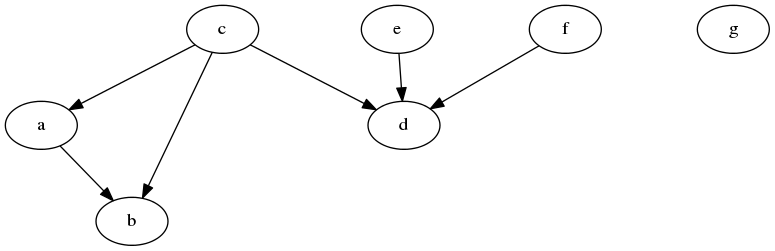
\includegraphics[width=.5\linewidth]{init.png}
	\caption{The initial graph from the book}
	\label{fig:init_graph}
	\end{figure}
	\begin{figure}[]
	\centering
	\begin{subfigure}{.5\textwidth}
	  \centering
	  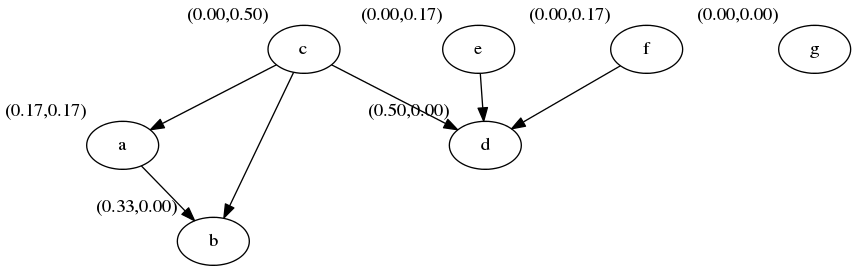
\includegraphics[width=\linewidth]{HITS_it1.png}
	  \caption{HITS iteration 1}
	  \label{}
	\end{subfigure}%
	\begin{subfigure}{.5\textwidth}
	  \centering
	  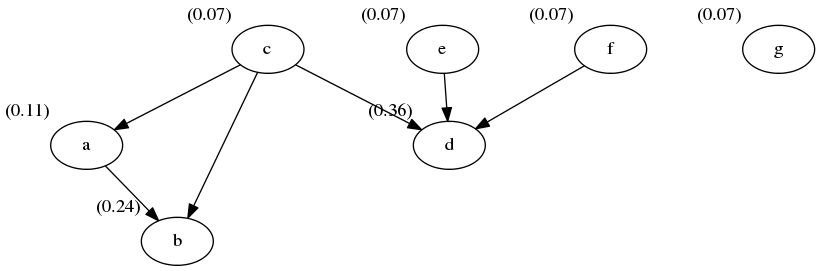
\includegraphics[width=\linewidth]{PR_graph_iter_1.png}
	  \caption{PageRank iteration 1}
	  \label{}
	\end{subfigure}
	\caption{Iteration 1 of the two algorithms}
	\label{fig:PR_HITS_it1}
	\end{figure}
	\begin{figure}[]
	\centering
	\begin{subfigure}{.5\textwidth}
	  \centering
	  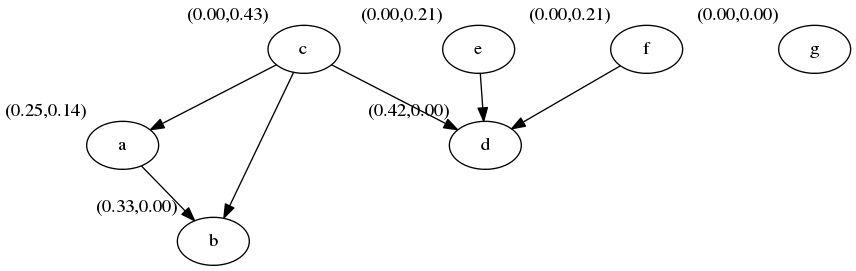
\includegraphics[width=\linewidth]{HITS_it2.png}
	  \caption{HITS iteration 2}
	  \label{}
	\end{subfigure}%
	\begin{subfigure}{.5\textwidth}
	  \centering
	  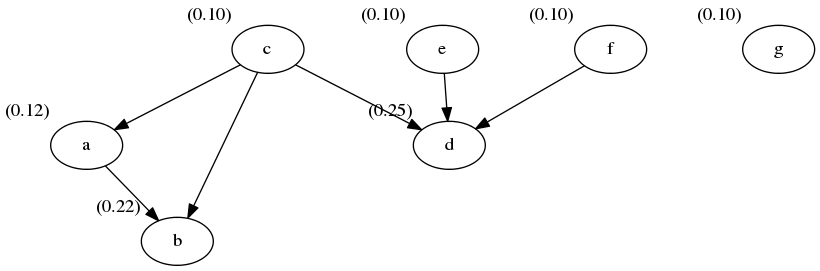
\includegraphics[width=\linewidth]{PR_graph_iter_2.png}
	  \caption{PageRank iteration 2}
	  \label{}
	\end{subfigure}
	\caption{Iteration 2 of the two algorithms}
	\label{fig:PR_HITS_it2}
	\end{figure}
	\begin{figure}[]
		\centering
		\begin{subfigure}{.5\textwidth}
		  \centering
		  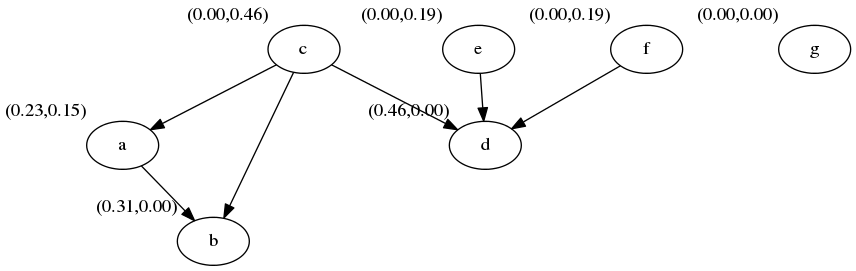
\includegraphics[width=\linewidth]{HITS_it3.png}
		  \caption{HITS iteration 3}
		  \label{}
		\end{subfigure}%
		\begin{subfigure}{.5\textwidth}
		  \centering
		  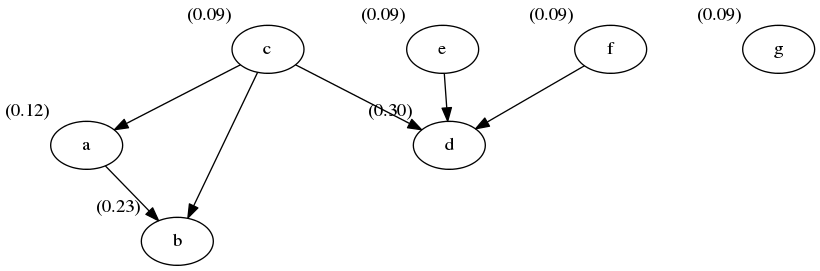
\includegraphics[width=\linewidth]{PR_graph_iter_3.png}
		  \caption{PageRank iteration 3}
		  \label{}
		\end{subfigure}
		\caption{Iteration 3 of the two algorithms}
		\label{fig:PR_HITS_it3}
	\end{figure}
	\begin{figure}[]
			\centering
			\begin{subfigure}{.5\textwidth}
			  \centering
			  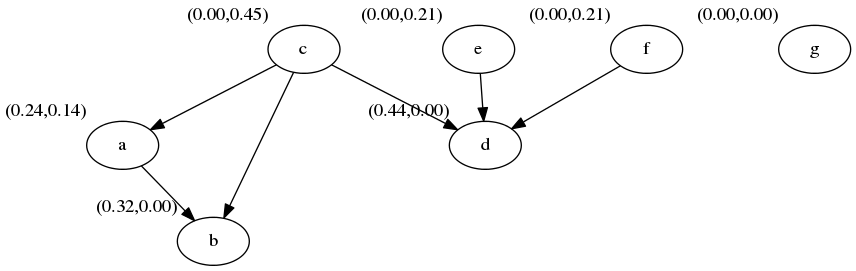
\includegraphics[width=\linewidth]{HITS_it4.png}
			  \caption{HITS iteration 4}
			  \label{}
			\end{subfigure}%
			\begin{subfigure}{.5\textwidth}
			  \centering
			  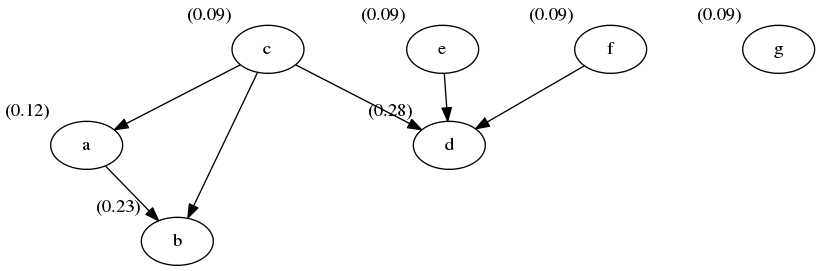
\includegraphics[width=\linewidth]{PR_graph_iter_4.png}
			  \caption{PageRank iteration 4}
			  \label{}
			\end{subfigure}
			\caption{Iteration 4 of the two algorithms}
			\label{fig:PR_HITS_it4}
	\end{figure}
	\begin{figure}[]
			\centering
			\begin{subfigure}{.5\textwidth}
			  \centering
			  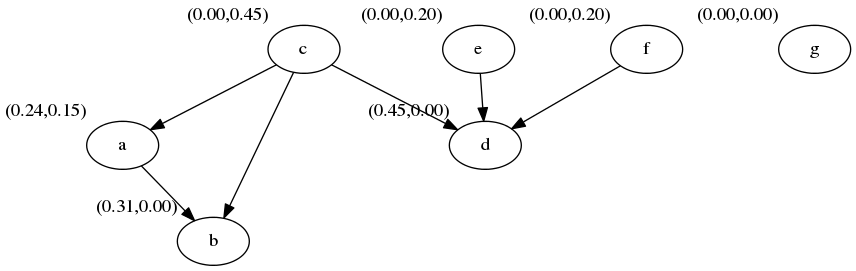
\includegraphics[width=\linewidth]{HITS_it5.png}
			  \caption{HITS iteration 5}
			  \label{}
			\end{subfigure}%
			\begin{subfigure}{.5\textwidth}
			  \centering
			  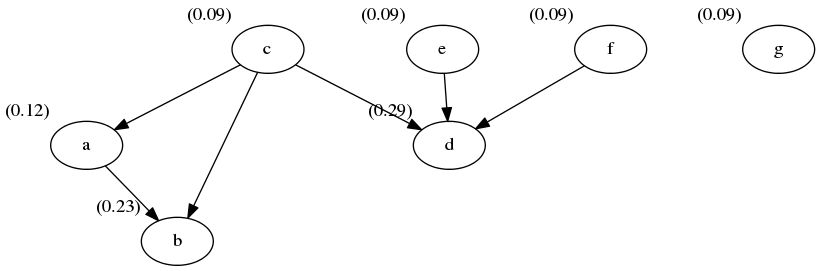
\includegraphics[width=\linewidth]{PR_graph_iter_5.png}
			  \caption{PageRank iteration 5}
			  \label{}
			\end{subfigure}
			\caption{Iteration 5 of the two algorithms}
			\label{fig:PR_HITS_it5}
	\end{figure}
We can see that the final ranking for both algorithms is the same as shown in table \ref{tb:rank_PR_HITS}. The scores in HITS are higher for the nodes that have at least one incoming link, however, the nodes that do not have any, are set to 0. And since PageRank sets a non-zero value to all nodes, including the ones without inlinks and the fact that the total score in both algorithms is 1, it makes sense that HITS scores are higher for the nodes with inlinks. The code for this question can be seen in listing \ref{lst:10_3} and the script to produce the pictures in listing \ref{lst:gen_pics}.
	\begin{table}[]
	\centering
	\caption{Node ranking based on PageRank and HITS algorithms}
	\label{tb:rank_PR_HITS}
	\begin{tabular}{|c|c|c|}
	\hline
	Node & PageRank & HITS \\ \hline
	a    & 3        & 3    \\ \hline
	b    & 2        & 2    \\ \hline
	c    & 4        & 4    \\ \hline
	d    & 1        & 1    \\ \hline
	e    & 4        & 4    \\ \hline
	f    & 4        & 4    \\ \hline
	g    & 4        & 4    \\ \hline
	\end{tabular}
	\end{table}
	\lstinputlisting[language=Python,caption={Script to generate the PageRank and HITS values for the given graph},label={lst:10_3}]{10_3.py}
	\lstinputlisting[language=Bash,caption={Bash script to generate the graphs with PageRank and HITS annotations},label={lst:gen_pics}]{gen_graph.sh}
	
\section*{Question 10.5}
Find a community-based question answering site on the Web and ask two questions, one that is low-quality and one that is high-quality. Describe the answer quality of each question.
\subsection*{Answer}
Since there are already so many bad and good questions on the internet, I decided not to post some new ones but instead just use some of the existing ones. Those had more time to collect answers and thus, I believe I will have a more reliable conclusion based on them. The low-quality question that I use for this assignment is  ``Y r u living?'' from Yahoo! answers. This looks quite bad to me. First of all, it doesn't even use full words to form the sentence, just some letters that sound the same as the words that should be there. Second, it's so general and does not really make any sense to ask this question. A sample of the answers to this question are:\\
\\``You must be a thicko to type on here in text language. \\You must work in WalMart where you do not need an education, you sounds ridiculous.''\\``Bcuz Itz betr thn the alternative''\\``for some reason i can't explain''\\
\\We see that the quality of the answers is low as well. I don't think that someone asking like that could expect a better answer than those. The answers mainly make fun of the question and one also uses a same way of excluding letters from the words. For the high-quality question I chose the question: \\``Do lambda expressions have any use other than saving lines of code?
Are there any special features provided by lambdas which solved problems which weren't easy to solve? '' from stackoverflow. I think that this question is understandable and to the point with correct spelling and grammar. That makes it a good question in my opinion. There were several long and good answers but I chose a smaller one that resembles them well.\\

``Programming languages are not for machines to execute. They are for programmers to think in.

Languages are a conversation with a compiler to turn our thoughts into something a machine can execute. One of the chief complaints about Java from people who come to it from other languages (or leave it for other languages) used to be that it forces a certain mental model on the programmer (i.e. everything is a class).

I'm not going to weigh in on whether that's good or bad: everything is trade-offs. But Java 8 lambdas allow programmers to think in terms of functions, which is something you previously could not do in Java.

It's the same thing as a procedural programmer learning to think in terms of classes when they come to Java: you see them gradually move from classes that are glorified structs and have 'helper' classes with a bunch of static methods and move on to something that more closely resembles a rational OO design (mea culpa).

If you just think of them as a shorter way to express anonymous inner classes then you are probably not going to find them very impressive in the same way that the procedural programmer above probably didn't think classes were any great improvement.'' The answer is precise, answers well the question asked and is very nicely constructed. We can see that the person that wrote this answer spend some time to think and form this answer in order to best convey to the other user his/her knowledge.

\section*{Question 10.6}
Find two examples of document filtering systems on the Web. How do they build a profile for your information need? Is the system static or adaptive?
\subsection*{Answer}
Nowadays, most of the leading websites use some kind of profiling system that is able to generate user profiles that are used to provide user-relevant content. For my two examples I used YouTube and Amazon. YouTube is the most popular video hosting website featuring millions of user uploaded videos. \\YouTube tracks the videos watched by each user and is then able to make recommendations on the main page, set the next to play video or recommend channels from creators that are supposed to create videos relevant to the user. One can clearly see the difference of the next video to play by accessing it through a freshly installed browser (or by deleting cookies) and not signing in. In this case, the next video is found looking at videos relevant to the previous one only.
\\Amazon is another top-traffic website. It consists an Internet marketplace where almost every product can be purchased. The filtering works by tracking the products a user visits and buys. It realizes correlations by the purchases that come together by users. When a user buys a set of products at the same transaction, it is quite propable that another user will also be interested in the other products of the set when checking one of them.
\\Both websites use adaptive filtering, since the preferences of their users may change from time to time, or expand to different areas.
\section*{Question SVMLight1}
Work through the ``Inductive SVM''example, discuss in detail the steps and resulting output.
\subsection*{Answer}

First I installed SVMLight from \url{http://www.cs.cornell.edu/people/tj/svm_light/}. Then I downloaded the example folder located at \url{http://download.joachims.org/svm_light/examples/example1.tar.gz}. The content of the examples is the training set examples. The first lines may contain comments and are ignored if they start with \#. Each of the following lin
es represents one training example and is of the following format:
	\begin{figure}[h]
			\centering
			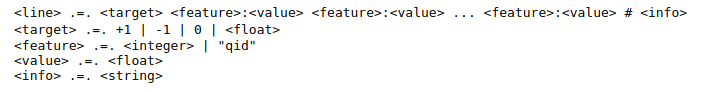
\includegraphics[width=\linewidth]{training_example.png}
		
			\label{fig:training_example}
	\end{figure}
\\The target value and each of the feature/value pairs are separated by a space character. Features with value zero can be skipped. The string info can be used to pass additional information to the kernel (e.g. non feature vector data).
In classification mode, the target value denotes the class of the example. +1 as the target value marks a positive example, -1 a negative example respectively.\\
Running the svm\textunderscore learn program as denoted on the Inductive example produced the model file used for the classification. The output of the svm\textunderscore learn is shown in figure \ref{fig:SVM_learn}.
	\begin{figure}[h]
			\centering
			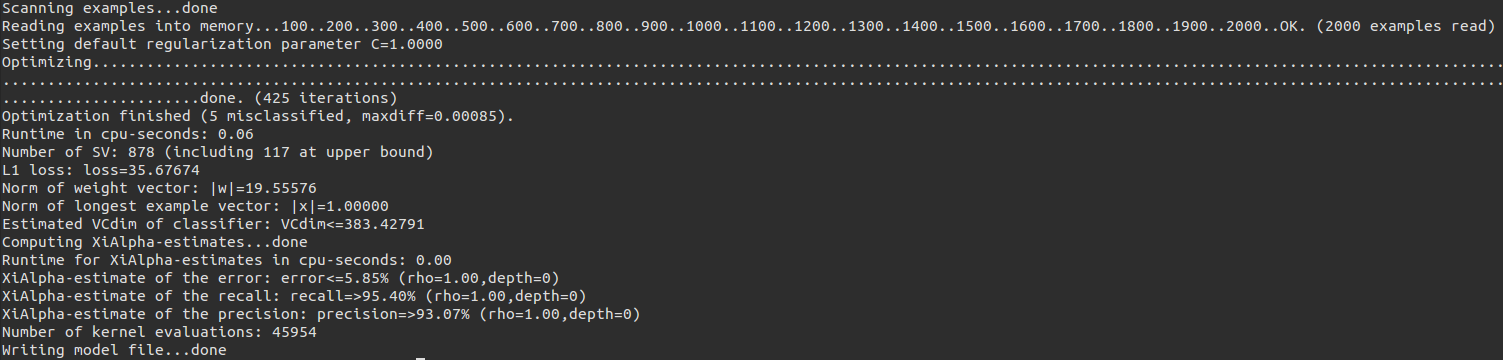
\includegraphics[width=\linewidth]{svm_learn.png}
			\caption{Output of the svm\textunderscore learn program}
			\label{fig:SVM_learn}
	\end{figure}
Once the model is generated, svm\textunderscore classify is run to perform the classification on the test set which consists of 600 examples. As seen in figure \ref{fig:SVM_classify}, the accuracy of the classifier was 97.67 having 14 incorrect results out of 600 tests. The precision on the set test was $96.43\%$ and the recall was $99\%$ 
\begin{figure}[h]
			\centering
			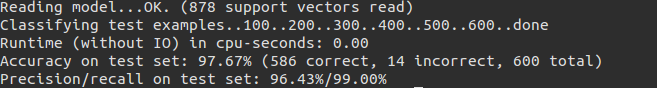
\includegraphics[width=\linewidth]{svm_classify.png}
			\caption{Output of the svm\textunderscore learn program}
			\label{fig:SVM_classify}
	\end{figure}
	\section*{Question SVMLight2}
	Create your own example modeled after the "Inductive SVM" example
	\begin{enumerate}
	\item pick a topic (e.g., "Australia") and provide 100 positive and 100 negative examples for training data:
		\begin{itemize}
		\item using the Reuters-21578 collection (linked from the SVMlight page) 
		\item or, create your own collection with crawled web pages
		\end{itemize}
	\item pick 30 documents not in the training set for your test data
	\item stem the words in the collection, using TFIDF as the features (compute for the 230 documents)
	\item train, classify, and discuss the results
	\end{enumerate}  
\subsection*{Answer}
To answer this question, I used nltk.corpus library and its Reuters-21578 collection.This library provides an API that can be used to extract the words, topics, raw text and other information about each of the documents. I picked as the word ``Oil''. To extract the 100 positive examples for training, I used the function that returns all the words in a document for each document in the collection and then checked if the word ``Oil'' is part of them. For the negative examples, I used the documents that did not include this word at all.\\ I kept the first 100 of the results for both cases as training set and another 15 from each one for the testing set. The TDIDF values of the features were then computed using the sklearn library and the tokenize function found in \ref{lst:reuters}. Once those values are computed for each document, the results are written in a file "train\textunderscore data.dat" for the training data and "test\textunderscore data.dat" for the testing data in the format SVMlight requires.\\ We can now use SVMLight to perform the training and the classifying using the files generated by the Python script. The output of the programs svm\textunderscore learn and svm\textunderscore classify can be seen in Figures \ref{fig:learn} and \ref{fig:classify}, respectively. 
\lstinputlisting[language=Python,caption={Script to generate the training and test data to feed SVMLight with},label={lst:reuters}]{reuters.py}

\begin{figure}[h]
			\centering
			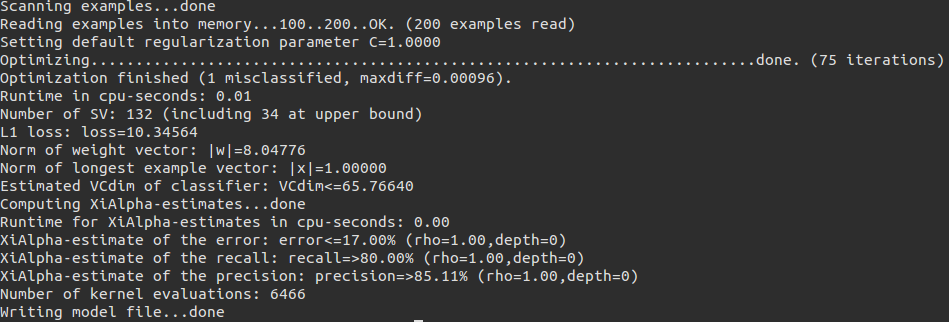
\includegraphics[width=\linewidth]{learn_oil.png}
			\caption{Output of the svm\textunderscore learn for the ``Oil'' topic}
			\label{fig:learn}
	\end{figure}
	\begin{figure}[h]
				\centering
				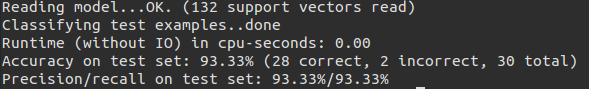
\includegraphics[width=\linewidth]{classify_oil.png}
				\caption{Output of the svm\textunderscore classify for the ``Oil'' topic}
				\label{fig:classify}
		\end{figure}
The precision estimation we get according to fig. \ref{fig:learn} is 85\%. The actual accuracy on the test data however, is 93\%, scoring 28 correct classifications out of 30 documents (fig. \ref{fig:classify}). 
\end{document}
